\documentclass[Report.tex]{subfiles}

\newcommand{\newaxis}[7]{
\begin{axis}[
    ybar,
    title={#1},
    ymin=#3, ymax=#4,
    bar width=1em,
    width={#5},
    height={#6},
    legend style={at={#7},anchor=north,legend columns=-1},
    enlarge x limits=0.4,
    x tick label style={align=center,text width=2cm},
    symbolic x coords={Logistic Regression, Random Forest, Multi-layer Perceptron},
    xtick=data,
    ylabel={#2}
]
}

% #1 - Feature name
% #2 - Metric name
\newcommand{\plotbar}[3] {
\addplot+[
	discard if not={features}{#1},
] table [x=model, y=#2, col sep=comma] {data/15-game-cv.csv};
\addlegendentry{#3}
}

%\pgfplotstableread[col sep=comma]{data/15-pair-cv.csv}\fifteenPairCV

\begin{document}

\section{Player identification}\label{sec:game-classification}
This section describes the methodology behind the first classification problem: \textit{Given a match of Dota 2, who is the player playing this hero?} The different experiments conducted are also detailed with discussion and analysis of their results. 



\subsection{Approach}\label{sec:game-approach}
To simplify the process and results, this approach took the view of looking at the question as a binary classification problem. This rephrases the question as: \textit{Given a match of Dota 2, is it player X playing this hero?} where player X is the chosen player to be matched on. All other players are simply considered as not player X. 

Particular attention is drawn to the exploration of the mouse movement features. While the game statistic and itemisation features output once for each match, for example total gold gained per minute, or the hashed encoding of inventory items is only output as one sample each, the mouse movement features created samples for every defined level 3 mouse action that a player makes, generating thousands of actions in a single match. As such, the exploration of mouse movement features was done in two different approaches. 

The first looked at using each individual action as a data point for training and testing. This means the context of what is a match is lost and it becomes a classification problem of individual mouse actions rather than a classification of matches. By encoding the data this way, a large number of training and testing samples were created, as all the actions were concatenated together. The results of this approach gave an indication to how useful individual actions are, and whether they can be used, or if further processing, such as grouping the actions into time slices was required or not. The second approach grouped all three types of mouse movement features in a single match together, which is representative of the classification problem of Dota 2 matches. 

% Each action was then tagged as one of two groups - is the player or is not the player. In this binary classification problem, only a single player is trained as one group and all other players as the other group. In this sense, the question being asked becomes \textit{given a level 3 action, is the player who performed this action player X?} Moreover, by encoding the data this way, a large number of training and testing samples are created from just a small number of games, as each game contained thousands of level 3 actions.

% The models therefore are training on each row and predicted whether a single action belonged to the player or not.

% In the second iteration, the mouse movement features are grouped together for each match. This gave the models each match as a data point, which is more representative of the problem of classifying a match of Dota 2.

\begin{figure}[H]
\pgfdeclarelayer{background}
\pgfdeclarelayer{foreground}
\pgfsetlayers{background,main,foreground}

% Block styles
\tikzstyle{data}=[draw, fill=blue!20, text width=5em, 
    text centered, minimum height=2.5em]
\tikzstyle{model} = [data, text width=5em, fill=red!20, 
    minimum height=3em, rounded corners]

\def\blockdist{3}
\newcommand{\newMoveModel}[3]{
    \node (#2-model) at (2,#3) [model] {#1 Model};
    \path (#2-model.west)+(-\blockdist,0) node (#2) [data] {#1 actions}; 
   
    \path (#2-model.east)+(\blockdist,0) node (#2-output) [data] {Predictions};
    
    \path [draw, ->] (#2.east) -- node {} (#2-model);
    \path [draw, ->] (#2-model.east) -- node{} (#2-output);
}

\newcommand{\newGameModel}[4]{
    \node (#2-model) at (2,#3) [model] {#1 Model};
    \path (#2-model.west)+(-\blockdist,0) node (#2) [data] {#4}; 
   
    \path [draw, ->] (#2.east) -- node {} (#2-model);
}
\begin{subfigure}{1\textwidth}
\centering
\begin{tikzpicture}
\newMoveModel{AC}{ac}{4}
\newMoveModel{MC}{mc}{2.5}
\newMoveModel{SC}{sc}{1}
\end{tikzpicture}
\caption{Classifying individual mouse actions}
\vspace{\baselineskip}
\end{subfigure}

\hspace{\fill}

\begin{subfigure}{1\textwidth}
\centering
\def\blockdist{2}
\begin{tikzpicture}
\newGameModel{AC}{ac}{4}{AC actions}
\newGameModel{MC}{mc}{2.5}{MC actions}
\newGameModel{SC}{sc}{1}{SC actions}
\newGameModel{Stats}{stats}{-0.5}{Game statistics}
\newGameModel{Items}{items}{-2.0}{Game items}

\path (sc-model.west)+(-6,0) node (game) [data] {Game};
\path (sc-model.east)+(2.5,0) node (combine) [model] {MLP};
\path (combine.east)+(2.5,0) node (output) [data] {Prediction};

\path [draw, ->] (game.20) -- node [above] {} (ac.180);
\path [draw, ->] (game.10) -- node [above] {} (mc.180);
\path [draw, ->] (game.0) -- node [above] {} (sc.180);
\path [draw, ->] (game.350) -- node [above] {} (stats.180);
\path [draw, ->] (game.340) -- node [above] {} (items.180);

\path [draw, ->] (ac-model.east) -- node [above] {} (combine.160);
\path [draw, ->] (mc-model.east) -- node [above] {} (combine.170);
\path [draw, ->] (sc-model.east) -- node [above] {} (combine.180);
\path [draw, ->] (stats-model.east) -- node [above] {} (combine.190);
\path [draw, ->] (items-model.east) -- node [above] {} (combine.200);

\path [draw, ->] (combine.east) -- node [above] {} (output);

\begin{pgfonlayer}{background}
  \path (ac.west |- ac.north)+(-0.5,0.5) node (a) {};
  \path (ac-model.south -| combine.east)+(+0.5,-0.5) node (b) {};
  \path (combine.east |- items-model.east)+(+0.5,-1) node (c) {};        
  \path[fill=yellow!20,rounded corners, draw=black!50, dashed] (a) rectangle (c);           
  \path (ac.north west)+(-0.2,0.2) node (a) {};        
\end{pgfonlayer}
\end{tikzpicture}
\caption{Classifying a single match}
\end{subfigure}
\caption{Difference between classifying each level 3 action and classifying each game. For the game classifier, each type of level 3 action is split per game and evaluated with separate models. This also allows new features to be easily added to the classifier in later stages. The probability of the separate models are then used for the combining model (MLP).}

\label{fig:game-classifier-difference}
\end{figure}

In order to combine the separate mouse actions from a match together, separate models were used to evaluate each type of level 3 action using the first approach. The results of the separate models are then combined by a simple multi-layer perceptron which takes the probability output of the models. The probability was chosen over the prediction to give the combining neural network a better range of values, rather than a binary output of the predicted class. The idea of using a simple network for the combination step is to be able to learn the relative weights for each type of mouse action, rather than use them all equally in a voting scheme, or set arbitrary weights to them. This does mean the network had to be trained in addition to training the separate models, but this is simply a small computational cost. Further, this approach is modular. Another approach would have been to simply concatenate all three types of mouse action together into one featureset, but it would not be scalable to the addition of more features. Further, features that have a greater number of features in proportion to others may dominate, for example the one hot encoding of items creates over 1800 binary features when there are only 114 mouse movement features in total. As such using a combination step allowed for better scalability and the addition of more features to be easily added as a separate model and input into the combining network.

The combining neural network was kept very simple in order to avoid complications with large hidden layers and activation functions, as its purpose was to learn and balance weights between the different features to give the best performance. It used a relu activation function and only contained one hidden layer with 3 neurons.


\subsection{Experimental design}\label{sec:game-experimental}
The features discussed in section \ref{sec:methodology} were initially explored individually to examine their performance. Where the features contained multiple approach or subtypes, such as the itemisation encoding and types of mouse actions, each was also explored individually to ascertain which approach performed better. As this approach used individual matches, the training and testing datasets were split carefully to ensure the testing set contained players and matches which do not appear in the training set, in order to eliminate potential data leakage. The one player used as the positive sample class was the only player which appeared in both training and testing sets. All the experiments used a two-step evaluation method to obtain metrics for training and testing.
\begin{enumerate}
\item During training, evaluation metrics were gathered using a 5-fold cross evaluation. This gives an idea on how well the models and feature perform, but the performance is likely inflated as the same players may appear in both the training and evaluation data. A 5-fold cross evaluation was chosen to give a balance between the amount of data used for training and evaluation (80\% and 20\% respectively for each fold) and performing enough runs to get a strong average. 
\item After the 5-fold cross evaluation, the final model is trained using all the training data, and evaluated against the testing data. This is the best indication of how the models perform against unseen data, as the testing data is untouched until this point of the experiment. 
\end{enumerate}
%Four
Three different models were used for evaluation. These models were chosen based on what was used in related work \cite{starcraft-identification, dota-gao, dota-eggert, mouse-dynamics} and to cover a range of different approaches. The three models are logistic regression, random forest and a neural network (in the form of a multi-layer perceptron).

Three performance metrics were used to evaluate the features and the machine learning models: accuracy, precision and recall. Each metric measured a different aspect of performance. 

\textbf{Accuracy} \\
Accuracy measured the overall performance of the model and feature by computing the total number of correct predictions over the total number of predictions.
\begin{equation*}
\text{accuracy} = \frac{\text{correct predictions}}{\text{total predictions}}
\end{equation*}
It is a simple measure that gives a good indication to the performance, but is relatively limited in what it can reveal. It can be inaccurate when the percentage of classes are unbalanced, as a model that predicts only the majority class will still achieve a high accuracy. Further, accuracy does not reveal additional detail about where misclassification occurs as it does not differentiate between false positives and false negatives. 

\textbf{Precision and Recall} \\
Precision and recall are complementary metrics that measure the relevance of predictions, with precision taking into account false positive results and recall taking into account false negative results. 
\begin{equation*}
\text{precision} = \frac{\text{true positives}}{\text{true positives} + \text{false positives}}
\end{equation*}

\begin{equation*}
\text{recall} = \frac{\text{true positives}}{\text{true positives} + \text{false negatives}}
\end{equation*}
In other words, precision helps identify the accuracy of positive predictions and recall helps identify the accuracy of predicting positive samples. These measures are useful to help narrow down why certain features or models may be behaving in a certain way. For example, a high recall but low precision suggests the model or feature is biased towards positive samples, as there are low false negatives but high false positives. 


\subsection{Mouse movement features}\label{sec:mm-features-results}

\subsubsection{Individual mouse actions}
When looking at the types of mouse movement features individually, a clear pattern can be seen in the performance of each type, and to a lesser extent the model used.

Generally, it can be seen from figure \ref{fig:move-results} that each type of mouse movement action (attack actions, move actions and spell cast actions) had differing performance irrespective of the model or metric used. The mouse movement following an attack action performed the best in every circumstance, while the mouse movement following a spell cast performed the worst. It must be noted that the number of each type of mouse action were not in proportion to the other types in each match. The average distribution of attacks, move, cast mouse actions in the dataset was 20\%, 78\% and 2\% respectively. This directly affects the number of data points for training and testing of each type of mouse action, making move command actions the most common and spell cast command actions the least. 
\begin{figure}[H]
%TODO replot this data with csv
\begin{subfigure}{1\textwidth}
\centering
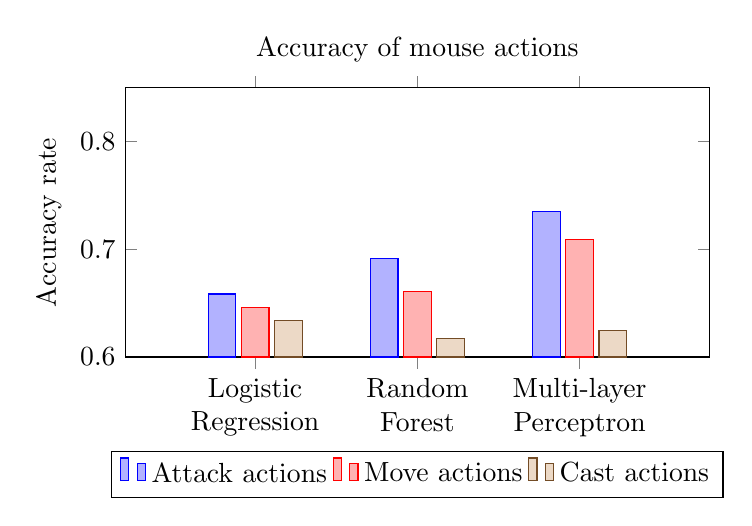
\begin{tikzpicture}
\newaxis{Accuracy of mouse actions}{Accuracy rate}{0.6}{0.85}{9cm}{5cm}{(0.5,-0.35)}
\addplot coordinates {(Logistic Regression,0.6586) (Random Forest,0.6915) (Multi-layer Perceptron,0.7355)};
\addplot coordinates {(Logistic Regression,0.6457) (Random Forest,0.6609) (Multi-layer Perceptron,0.7094)};
\addplot coordinates {(Logistic Regression,0.6339) (Random Forest,0.6173) (Multi-layer Perceptron,0.6248)};
\legend{Attack actions, Move actions, Cast actions}

\end{axis}
\end{tikzpicture}
\end{subfigure}

\begin{subfigure}{0.45\textwidth}
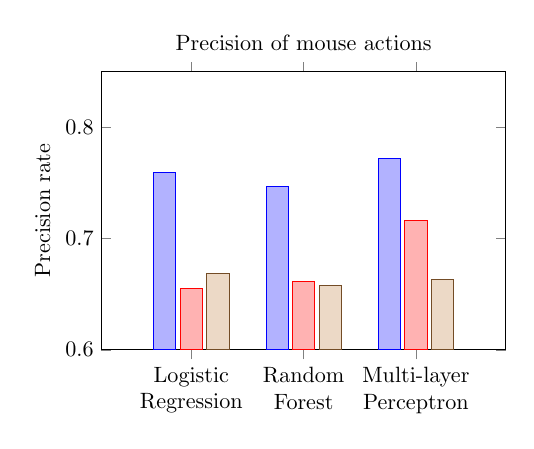
\begin{tikzpicture}[scale=0.8]
\newaxis{Precision of mouse actions}{Precision rate}{0.6}{0.85}{8cm}{6cm}{(0.5,-0.25)}

\addplot coordinates {(Logistic Regression,0.759) (Random Forest,0.747) (Multi-layer Perceptron,0.7719)};
\addplot coordinates {(Logistic Regression,0.65524) (Random Forest,0.6618) (Multi-layer Perceptron,0.7165)};
\addplot coordinates {(Logistic Regression,0.6683) (Random Forest,0.6582) (Multi-layer Perceptron,0.6633)};
%\legend{Attack,Move,Cast}

\end{axis}
\end{tikzpicture}
\end{subfigure}
\hspace{\fill}
\begin{subfigure}{0.45\textwidth}
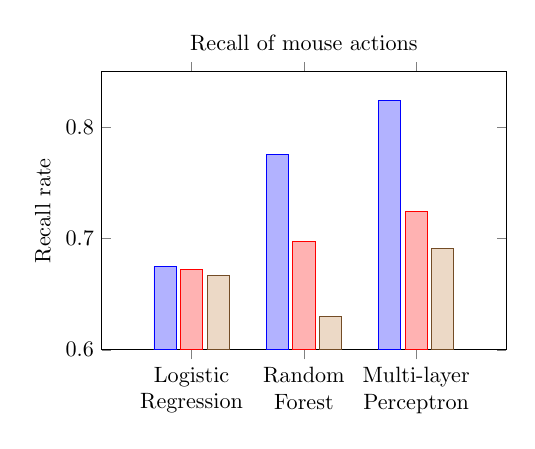
\begin{tikzpicture}[scale=0.8]
\newaxis{Recall of mouse actions}{Recall rate}{0.6}{0.85}{8cm}{6cm}{(0.5,-0.25)}
\addplot coordinates {(Logistic Regression,0.6747) (Random Forest,0.7754) (Multi-layer Perceptron,0.8243)};
\addplot coordinates {(Logistic Regression,0.672) (Random Forest,0.6975) (Multi-layer Perceptron,0.7239)};
\addplot coordinates {(Logistic Regression,0.6665) (Random Forest,0.6301) (Multi-layer Perceptron,0.6909)};
%\legend{Attack,Move,Cast}
\end{axis}
\end{tikzpicture}
\end{subfigure}
\caption{Classification rates using only mouse movement features.}
\label{fig:move-results}
\end{figure}

Taking this into account, mouse movement features from attack commands make a strong case for being the most effective at predicting player behaviour. This can be seen especially in the case of precision and recall rate. This demonstrates a low false positive and false negative rate and shows that every individual mouse action that a player takes contains some unique behaviour that help differentiate it from another player's mouse actions. 

There is a good explanation for these results and why the mouse dynamics of a player are more unique from attack commands compared to the other two. Firstly, the number of movement commands are the highest, as they are the most common command for players to send in a match, typically in the order of a few thousand move commands. This is partly because movement and position is the most fundamental part of Dota 2, and as a progression to this, most players move (or right-click) their heroes constantly, multiple times a second. There are many reasons for this behaviour, but this constant moving can lead difficulty in distinguishing between different players, as the mouse movement between each move command is very short. 

Secondly the chosen hero in the dataset is a hero called Razor, which was not a good example for a spell casting hero, as only one of his four spells is targeted, meaning the mouse movements captured during spell cast are likely to contain a lot of noise, as two of his other abilities activate without a target. Despite this oversight, it is good to see that for such a hero, spell cast movements are less useful while attack movements are more useful. Finally, mouse movements following attack commands happen frequently, both during laning phase for hitting neutral creeps, and during later stages of a match during teamfights while not being over saturated like move commands, which allows a lot of data points that are more unique compared to the move commands. 

\begin{figure}[H]
\caption{confusion matrix of attack mouse movements with mlp}
\end{figure}

The classification rate itself was also strong, with attack mouse movements using a neural network achieving 73\% accuracy and high precision and recall. (TODO numbers of confusion matrix) With these positive results, no additional pre-processing or fine grained parsing was necessary to progress with investigating the use of different mouse movement types together to classify a match.


\subsubsection{Mouse movements for each match}\label{sbsec:game-classification}
When all three types of mouse action are grouped together, a different pattern emerges. 

\begin{figure}[H]
\centering
\begin{tikzpicture}
\newaxis{\textbf{Classifying matches with mouse movements combined}}{Metric rate}{0.1}{1.03}{9cm}{6cm}{(0.5,-0.27)}

\plotbar{mouse}{accuracy}{Accuracy}
\plotbar{mouse}{precision}{Precision}
\plotbar{mouse}{recall}{Recall}

\end{axis}
\end{tikzpicture}
\caption{Training results of classifying each match with all three types of mouse actions combined. Note that the size of the dataset is reduced significantly compared to the approach where mouse actions were used individually.}
\end{figure}


The accuracy of the random forest classifier drops while it gets perfect precision. This is indicative of an issue in the predictions, as perfect precision means no false positives while the low recall suggests a lot of false negatives. The picture becomes clearer by looking at the confusion matrix of predictions. Table \ref{tbl:rf-mouse-confusion-matrix} shows 0 false positives predicted and a very large proportion of false negatives. This shows there is an issue with the random forest classifier, as it predicts negative values very often. Moreover, there are still a few true positive predictions, which means the model is not predicting only negatives. This seems to show a specific player's (the positive sample) behaviour is difficult to differentiate from another player in many cases, but when it can be detected it is very obviously from the specific player. 

\begin{table}[H]
\centering
\begin{tabular}{| c | c |}
\hline
\makecell{True positives \\ 16} & \makecell{False positives \\ 0} \\ \hline
\makecell{False negatives \\ 39} & \makecell{True negatives \\ 44} \\ \hline
\end{tabular}
\caption{Confusion matrix of prediction samples from testing data for the random forest using only mouse movement features.}
\label{tbl:rf-mouse-confusion-matrix}
\end{table}

Aside from the random forest results, the performance of logistic regression was quite noteworthy, as it matches the neural network in all three performance metrics. This is an improvement compared to training on mouse movements individually, as logistic regression had lower recall which hurt its accuracy. Keep in mind that the models are used only when training each individual mouse action as before, and the combination step is another neural network (see figure \ref{fig:game-classifier-difference}). This means that despite the lower accuracy of logistic regression when classifying individual mouse movements, the combining network was able to learn the weights to apply to each of the three logistic regression models used to predict individual mouse movements. 

The difference in accuracy from each individual mouse actions and all mouse actions in a match demonstrate that there is a mixture of mouse actions that correlates to player behaviour. The usage of all mouse actions in a match allow the prediction of who the player is to be better refined. However, given the number of actions that occur in a match, it is interesting that the accuracy is not significantly higher, as the difference is only about 10\% more accuracy. This shows a limitation to predicting a player's behaviour using purely their mouse movement, likely a result of a lot of noise or certain mouse movement sequences that are less useful that others. More work into fine-grained data of each mouse action and the surrounding context of the match at the point where the actions are captured would be required to get a better picture of which exact actions are useful for prediction, and which actions are only adding noise to the prediction model. 



while random forest performed poorly in comparison. Most notably, the recall rate for the random forest classifier is only about 12\%. This is a sign that it predicted a large proportion of false negatives compared to the number of true positives and false positives, so the model was predicting that matches were not from the chosen player wrong. 

% Logistic regression is a linear model, suggesting linear relation between the player and the mouse movement data


\subsection{Game statistic features}
When looking at game statistics features only, a different trend arises. The logistic regression and random forest models perform exceptionally well while the neural network doesn't. In fact, the random forest gets close to perfect accuracy, precision and recall. 

\begin{figure}[H]
\centering
\begin{tikzpicture}
\newaxis{\textbf{Classifying matches with game statistics}}{Metric rate}{0.2}{1.03}{9cm}{6cm}{(0.5,-0.27)}

\plotbar{stats}{accuracy}{Accuracy}
\plotbar{stats}{precision}{Precision}
\plotbar{stats}{recall}{Recall}

\end{axis}
\end{tikzpicture}
\caption{Training results of classifying each match with game statistics.}
\end{figure}

This result is very suspicious, and so deserves a more in-depth look into why random forest was able to predict perfectly, and why the neural network performed so poorly. First, the cross validation of the random forest classifier was run with a higher and lower value of $k$. A higher number of $k$ allows for more trials to confirm if the result can be repeated for additional trials and the lower number of $k$ uses less training data, to see if it can continue to achieve good results using less data. 

\newcommand{\rfplotbar}[2] {
\addplot+[mark=none] table [x=cv, y=#1, col sep=comma] {data/15-game-rf.csv};
\addlegendentry{#2}
}
\begin{figure}[H]
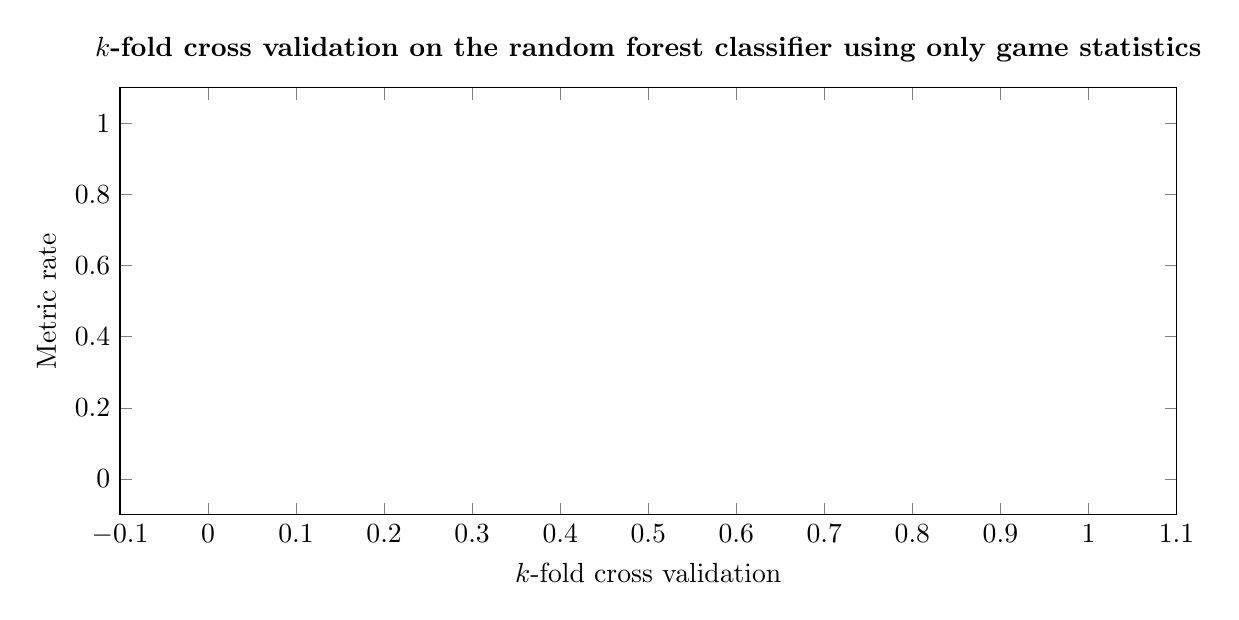
\begin{tikzpicture}
\begin{axis}[
    %ybar,
    title={\textbf{$k$-fold cross validation on the random forest classifier using only game statistics}},
    %ymin=#3, ymax=#4,
    %bar width=1em,
    width={15cm},
    height={7cm},
    legend style={at={(0.5,-0.2)},anchor=north,legend columns=-1},
    enlarge x limits=0.1,
    x tick label style={
        /pgf/number format/1000 sep=
    },
    %symbolic x coords={Logistic Regression, Random Forest, Multi-layer Perceptron},
    xtick=data,
    ylabel={Metric rate},
    xlabel={$k$-fold cross validation}
]

\rfplotbar{accuracy}{Accuracy}
\rfplotbar{precision}{Precision}
\rfplotbar{recall}{Recall}

\end{axis}
\end{tikzpicture}
\caption{Varying degrees of $k$-fold cross validation was run to determine if the random forest continues to obtain such good results.}
\end{figure}

Even when using a range of $k$ values for cross-validation, the performance metrics of the random forest classifier did not fall by much, which gives the perfect prediction result merit. The lowest accuracy obtained was 95\% with a 2-fold cross validation, meaning half the data was used for training and half the data for testing. 

%TODO look at testing data

%TODO why mlp is so bad for this


\subsection{Itemisation features}

All itemisation encoding methods performed similarly well with a few small differences. Many patterns are repeated across the three different models, which is a strong sign of the common strengths and weaknesses of each encoding method. 

Firstly, encoding boots only data had the lowest accuracy compared to the other methods in all three models. This shows the loss of data from only using boots have an impact on the ability to predict who the player is. That is not to say it is necessarily an inferior method as it loses some accuracy in exchange for using a lot less features. For comparison, the one-hot encoding of only starting items gets 4\%, 6\% and 7\% more accuracy for each model respectively, but uses 186 features compared to the 42 features of only encoding boots data. 

\begin{figure}[H]
\centering
\begin{tikzpicture}
\newaxis{\textbf{Accuracy of itemisation features}}{Accuracy rate}{0.7}{1.03}{12cm}{5cm}{(0.5,-0.27)}

\plotbar{items-hashed}{accuracy}{Items hashed}
\plotbar{items-onehot}{accuracy}{One-hot encoding}
\plotbar{items-starting}{accuracy}{Starting items}
\plotbar{items-select}{accuracy}{Boots only}
\legend{};
\end{axis}
\end{tikzpicture}

\begin{tikzpicture}
\newaxis{\textbf{Precision of itemisation features}}{Precision rate}{0.7}{1.03}{12cm}{5cm}{(0.5,-0.27)}

\plotbar{items-hashed}{precision}{Items hashed}
\plotbar{items-onehot}{precision}{One-hot encoding}
\plotbar{items-starting}{precision}{Starting items}
\plotbar{items-select}{precision}{Boots only}
\legend{};
\end{axis}
\end{tikzpicture}

\begin{tikzpicture}
\newaxis{\textbf{Recall of itemisation features}}{Recall rate}{0.7}{1.03}{12cm}{5cm}{(0.5,-0.35)}

\plotbar{items-hashed}{recall}{Items hashed}
\plotbar{items-onehot}{recall}{One-hot encoding}
\plotbar{items-starting}{recall}{Starting items}
\plotbar{items-select}{recall}{Boots only}

\end{axis}
\end{tikzpicture}
\caption{Accuracy, precision and recall for the different itemisation encoding methods.}
\end{figure}

The one-hot encoding of all items and just starting items had very similar performance, with starting items only getting better accuracy with the random forest and multi-layer perceptron models while all items had better accuracy on logistic regression. Recall that the encoding of all items is sampled twice in a match, once at the beginning and once at the end. In other words, the sample at the beginning of a match gives almost the same data as encoding starting items only, the difference being over a thousand binary features with a 0 value. The close performance of the two encoding methods suggests a few things. First is that the massive increase in binary features does not heavily impact performance. The encoding of all items contains about 9 times the number of features (281 items vs 31 items) but the accuracy deviates by less than 5\%. Next, the items in the inventory at the end of the match is the additional data that encoding starting items loses, yet only using starting items still does better in two of the three models. This shows the slot locations of starting items is more useful in player prediction than the items at the end of a match. The better performance may come from the narrower scope that starting items cover, which prevents noise that may affect prediction performance. This also makes sense from the game's perspective, as the items a player buys is often dependent on the strategy and composition of their own team and the opponent team. Further, many matches end before a player finishes buying all items they need, so the item locations recorded at the end of a match could be temporary and different from other matches by the same player, depending on the context of the match. 

Another point of interest is the performance of the hashed encoding method, which was surprisingly good and unexpected. In a way, hashing the items is the best method of encoding, as it precisely records which item was at which inventory slot with a smaller impact of the implied ordinal relation between the items as the hash is split into multiple features. However, it does not remove this implied relationship which in theory would result in poor performance. Nonetheless, it is not the case here, as the hashed encoding outperformed the one-hot encoding in every model even as both methods encoding the exact same information. 

%TODO recall has same pattern for all three models, but not precision

\subsection{Combining features}

A quick overview of all the featuresets individually with the three models shows how some features and models work better in different combinations, and some are more consistent. 

\begin{figure}[H]
\centering
\begin{tikzpicture}
\newaxis{\textbf{Accuracy of individual featuresets}}{Accuracy rate}{0.3}{1.03}{12cm}{5cm}{(0.5,-0.35)}

\plotbar{mouse}{accuracy}{Mouse movement}
\plotbar{stats}{accuracy}{Game statistics}
\plotbar{items-hashed}{accuracy}{Items hashed}
\plotbar{items-starting}{accuracy}{Starting items}

\end{axis}
\end{tikzpicture}
\caption{A comparison of the featuresets used individually to show which was able to predict the identity of the player in the dataset. }
\end{figure}

The itemisation data is the most consistent overall among the three models, as the mouse movement and statistics data obtain different accuracy depending on the model. The logistic regression model is also the most consistent for all the featuresets as the random forest and multi-layer perceptron have varied performance for mouse movement and game statistics. 

%This may come from player identification being a linear and relatively simple problem that the complicated models overfit/underfit. 

When combining the featuresets together in different combinations, a few interesting results are produced. 

\begin{table}[H]
\begin{tabular}{ c | c | c | c }
& \multicolumn{3}{c}{\textbf{Models}} \\ \hline
\textbf{Features} & Logistic Regression & Random Forest & Multi-layer Perceptron \\ \hline
Mouse & 0.859 & 0.595 & 0.848 \\ \hline
Stats & 0.959 & 1.0 & 0.484 \\ \hline
Items hashed & 0.929 & 0.888 & 0.929 \\ \hline
Items one-hot & 0.909 & 0.877 & 0.899 \\ \hline
Starting items & 0.899 & 0.919 & 0.939 \\ \hline
Boots only & 0.859 & 0.859 & 0.869 \\ \hline
Mouse + Stats & 0.959 & 0.597 & \textcolor{red}{0.738} \\ \hline
Mouse + Items hashed & 0.919 & 0.646 & 0.909 \\ \hline
Mouse + Items one-hot & 0.888 & 0.606 & 0.939 \\ \hline
Mouse + Starting items & 0.918 & 0.617 & 0.919 \\ \hline
Mouse + Boots only & 0.9109 & 0.857 & 0.908 \\ \hline
Stats + Items hashed & 0.969 & \textcolor{red}{0.990} & \textcolor{red}{0.868} \\ \hline
Stats + Items one-hot & 0.969 & \textcolor{red}{0.979} & \textcolor{red}{0.939} \\ \hline
Stats + Starting items & 0.959 & \textcolor{red}{1.0} & \textcolor{red}{0.929} \\ \hline
Stats + Boots only & 0.99 & \textcolor{red}{0.959} & \textcolor{red}{0.859} \\ \hline
Mouse + Stats + Items hashed & 0.949 & 0.636 & 0.808 \\ \hline
Mouse + Stats + Items one-hot & \textcolor{red}{0.726} & 0.769 & 0.919 \\ \hline
Mouse + Stats + Starting items & 0.959 & 0.586 & 0.929 \\ \hline
Mouse + Stats + Boots only & 0.959 & 0.615 & 0.928 \\
\end{tabular}
\caption{Accuracy of each model on each feature combination. The accuracies highlighted in red are particularly interesting as they break from a general trend in model performance.}
\end{table}

Logistic regression continued to perform well when the features are combined, but none are significantly better compared to using each featureset individually. Using game statistics and boots only encoding allowed the logistic regression model to achieve 99\% accuracy, which is odd as the boots only encoding had the lowest accuracy of all item encoding methods for logistic regression. Furthermore, using mouse movement, game statistics and one-hot encoding of all items led to a drastic reduction in accuracy in an odd anomaly.  

The random forest results are also very interesting, and show reduced results in most combinations compared to the individual features. For example, the mouse movement feature had a 60\% accuracy while the various itemisation encoding methods had about 85-90\% accuracy. When the movement feature was combined together with the itemisation features, 3 combinations only achieved 60-65\% accuracy while the boots only combination with mouse movement achieved about the same accuracy as the boots feature by itself. A similar pattern is observed when all three featuresets are combined together, as the accuracy stays quite low with all the additional features. The case is also true for the combination of game statistics and itemisation, though it is a difficult comparison as the game statistics alone had perfect predictions. In general for random forests, the addition of the mouse movement features was a big factor in the poor performance when combining features. This is likely related to the perfect precision but low recall described earlier for mouse movement features on the random forest classifier. What is interesting, is the addition of game statistics, which did not hinder predictions when combined with itemisation data, could not help raise accuracies higher when combined with mouse movement features. In fact the itemisation features helped raise accuracies much more than the statistic features did. This helps to suggest itemisation is one of the stronger indicators and can be combined with other features without introducing noise. %Something about RF properties makes it bad?

Finally, the simple neural network model had little issues when combining features together, but gained little advantages as well. As it performed poorly when using only statistics, the addition of mouse movement and itemisation was able to help boost accuracies. 


%TODO cite starcraft, feature + model matters, but items able to be good regardless

%TODO lr also most consistent for performance, shows maybe its a linear problem that the non-linear models over complicate, leading to over/underfitting


\subsection{Findings (conclusion)}

\end{document}
